% =============================================================================
%  arquivo_experimentos.tex — material retirado temporariamente do main.tex
% =============================================================================
%
%  Motivo do corte: reduzir o artigo ao escopo da multiplicacao de matrizes
%  (analise de ISA + isolamento do efeito do L1) antes de reintegrar o resto.
%  NADA aqui foi descartado: cada bloco esta integral, na ordem original.
%
%  Como devolver um bloco ao texto: no main.tex existe um marcador
%      %%% <<<REMOVIDO:ROTULO>>>
%  na posicao exata de onde o bloco saiu. Basta trocar o marcador pelo bloco
%  correspondente deste arquivo e renumerar os experimentos.
%
%  Ao reintegrar, conferir tambem:
%    - a numeracao dos experimentos (hoje 1 e 2; eram 1 e 3);
%    - o resumo/abstract, que foi reduzido as conclusoes que sobraram;
%    - a Conclusao, idem;
%    - as figuras fig_pchase_flags.png e fig_tdiv_ws.png, so referenciadas aqui.
%
% =============================================================================


%% =====================================================
% BLOCO: MET-EXP2-PCHASE
%% =====================================================

\subsection{Experimento 2: P-chase (Pointer Chasing)}

Para mapeamento direto das latências por nível de \textit{cache}, é implementado um microbenchmark baseado na técnica de \textit{pointer chasing} proposta por Wong et al.~\cite{wong2010} e refinada por Mei e Chu~\cite{mei2017}. O experimento percorre uma lista encadeada com permutação aleatória, variando o tamanho do \textit{working set} de 1~KB a 8~MB. Duas fases são conduzidas: (1)~\textit{single work-item} --- mede a latência pura sem contenção; e (2)~\textit{multi work-item} --- executa uma instância por CU (36 instâncias simultâneas), forçando contenção no L2 compartilhado e revelando a transição L2$\to$VRAM.

%% =====================================================
% BLOCO: MET-EXP4-7
%% =====================================================

\subsection{Experimento 4: Níveis de \textit{Cache} \textit{versus} Padrão de Acesso}

Confirmada a possibilidade de emitir \textit{flags} explicitamente, verificou-se que as quatro combinações de \textit{flags} de coerência são geradas corretamente no gfx803: \texttt{DC500000} (GLC=0, SLC=0), \texttt{DC510000} (\texttt{glc}), \texttt{DC520000} (\texttt{slc}) e \texttt{DC530000} (\texttt{glc slc}). No formato FLAT do GFX8, o bit~16 corresponde a GLC e o bit~17 a SLC.

Este experimento cruza os níveis de \textit{cache} com três cargas de fatores de reúso muito distintos, de modo a testar a hipótese de que o valor de um \textit{cache} depende do reúso temporal do padrão de acesso: \textit{streaming} puro (reúso~1, acesso coalescido em que cada elemento é lido uma única vez em todo o \textit{grid}), \textit{stencil} 2D \textit{blur} $3\times3$ (reúso~9, cada entrada participa de nove saídas) e multiplicação de matrizes \textit{naive} (reúso~$N$). As variantes de cada carga são geradas por macro a partir do mesmo código-fonte, diferindo exclusivamente na \textit{string} do modificador de \textit{cache}.

Como referência complementar, mede-se ainda uma redução sobre 16~MB sob três padrões de acesso à memória global --- sequencial contíguo, \textit{stride} fixo de 67 elementos e aleatório por \textit{xorshift} ---, com 262.144 \textit{work-items} e 128 iterações, mantidas as mesmas \textit{flags} de coerência em todos eles.

As saídas dos blocos de \textit{assembly} utilizam a restrição \textit{earlyclobber} (\texttt{"=\&v"}): sem ela, o compilador pode alocar um registrador de saída sobre um registrador de endereço ainda não consumido por um \textit{load} posterior do mesmo bloco, o que corrompe o endereço e provoca falha de página na GPU de forma reproduzível.

\subsection{Experimento 5: P-chase com Controle de Nível de \textit{Cache}}

O Experimento~4 mede vazão, o que não permite distinguir duas hipóteses sobre a \textit{flag} \texttt{slc}: (H1)~o L2 contribui pouco além do que o L1 já captura nessas cargas; ou (H2)~\texttt{SLC=1} não é \textit{bypass} rígido do L2. Para decidir entre elas, o microbenchmark P-chase do Experimento~2 é repetido sob as três configurações de \textit{flags}.

A medida decisiva é o \textit{working set} de 1~KB: um conjunto desse tamanho cabe folgadamente no L1 (16~KB) e no L2 (2~MB), de modo que a latência observada identifica sem ambiguidade qual nível serve o acesso. O método tem ainda uma vantagem sobre os Experimentos~3 e~4: como cada \textit{load} depende do anterior, a serialização é intrínseca e o \texttt{s\_waitcnt} do bloco de \textit{assembly} não acrescenta efeito algum --- o fator confundido desaparece por construção.

\subsection{Experimento 6: Scan, Primos e Crivo}

Para verificar se as conclusões se sustentam fora das cargas sintéticas, o controle de nível de \textit{cache} é aplicado a três algoritmos clássicos: \textbf{scan} (soma de prefixos em três fases, com reúso interno no LDS); \textbf{primos por divisão sucessiva}, incluído como \textbf{controle negativo} por ser \textit{compute-bound} (um \textit{load} por work-item e centenas de operações de ALU); e \textbf{crivo de Eratóstenes segmentado}, no qual a tabela de primos pequenos (2,2~KB) é percorrida por todos os work-items. Todos os resultados são verificados contra referência em CPU.


\subsection{Experimento 7: Densidade de \textit{Loads} e a Fronteira do L1}

O Experimento~6 registrou efeito nulo nos três algoritmos e atribuiu o resultado do crivo à uniformidade do acesso à tabela de primos. Este experimento testa essa atribuição trocando a \textbf{formulação} do teste de primalidade, sem trocar o problema: em vez do crivo segmentado, emprega-se \textbf{divisão sucessiva tabelada}, em que cada \textit{work-item} testa um candidato contra todos os primos ímpares até $\sqrt{v_{\max}}$.

O teste de divisibilidade usa a forma exata de Granlund e Montgomery~\cite{granlund1994}: para $p$ ímpar, $p \mid v$ se e somente se $v \cdot (p^{-1} \bmod 2^{32}) \le \lfloor (2^{32}-1)/p \rfloor$, com o inverso pré-computado no anfitrião. O custo por primo é de \textbf{dois \textit{loads} e cerca de cinco instruções de ALU}, sem divisão inteira --- que no GCN custa cerca de 25 instruções e devolveria o \textit{kernel} ao regime \textit{compute-bound} do controle negativo. O \textit{trip count} é fixo, de modo que não há divergência entre \textit{lanes}.

Três variantes isolam os fatores. Elas executam trabalho idêntico, o mesmo número de \textit{loads} e o mesmo número de iterações, diferindo apenas no índice inicial de cada \textit{lane} na tabela: \textbf{uniforme} (todos os \textit{lanes} no mesmo endereço, replicando o padrão do crivo), \textbf{dispersa} ($37\ell \bmod n$, com os 64 \textit{lanes} em posições distintas) e \textbf{dessincronizada} (o índice inicial varia também por \textit{work-group}, pela constante de Knuth $2^{32}/\varphi$). A terceira é necessária porque, avançando todos em \textit{lock-step}, as \textit{wavefronts} de uma mesma CU percorrem a tabela em fase e a janela viva permanece em torno de 4~KB, qualquer que seja o tamanho da tabela.

Numa segunda etapa, o conjunto de trabalho reusado é varrido de 2~KB a 51~KB mantendo o total de \textit{loads} constante em cerca de 640~M. A tabela contém os $k$ primeiros primos ímpares e os candidatos situam-se em $[\,\mathrm{lim}^2 - n,\ \mathrm{lim}^2)$, de modo que todo fator primo de qualquer candidato esteja na tabela e o teste permaneça exato. O limite superior de 51~KB decorre da aritmética de 32 bits, que exige $\mathrm{lim} < 65536$. Todos os resultados são verificados contra referência em CPU por divisão inteira --- técnica independente da empregada no \textit{kernel}.

%% =====================================================
% BLOCO: RES-EXP2-PCHASE
%% =====================================================

\subsection{Experimento 2: P-chase}

A Tabela~\ref{tab:pchase} resume os resultados do P-chase em modo \textit{single work-item} (latência pura, sem contenção entre CUs).

\begin{table}[ht]
\centering
\caption{Latência por \textit{working set} (P-chase, \textit{single work-item}).}
\label{tab:pchase}
\small
\begin{tabular}{@{}rrl@{}}
\toprule
\textbf{Working Set} & \textbf{Latência (ns)} & \textbf{Nível inferido} \\
\midrule
1--16 KB & 38,6--38,8 & L1 \\
20 KB & 59,0 (+52\%) & Transição L1$\to$L2 \\
24--256 KB & 70--130 & L2 \\
512 KB--32 MB & 139--256 & Transição L2$\to$VRAM (gradual) \\
\bottomrule
\end{tabular}
\end{table}

O salto de latência em 20~KB confirma experimentalmente que o \textit{cache} L1 da Ellesmere possui 16~KB por CU, consistente com a especificação da AMD. No modo \textit{multi work-item} (36 instâncias, uma por CU), a transição L2$\to$VRAM torna-se visível: a latência salta de 203~ns (\textit{working set} de 64~KB/CU, \textit{footprint} total de 2,3~MB $\approx$ L2) para 301~ns (256~KB/CU, \textit{footprint} de 9~MB $\gg$ L2), um aumento de $\sim$48\%. A VRAM sob contenção real (36 CUs simultâneos) apresenta latência 2,3$\times$ maior que no teste com 1 \textit{work-item}, evidenciando o efeito da contenção no barramento de memória.

%% =====================================================
% BLOCO: RES-EXP4-7
%% =====================================================

\subsection{Experimento 4: Níveis de \textit{Cache} \textit{versus} Padrão de Acesso}
\label{sec:niveis}

A Tabela~\ref{tab:reuso} apresenta o custo de contornar o L1 para as três cargas.

\begin{table}[ht]
\centering
\caption{Custo de contornar o L1 (\texttt{glc}) em função do reúso do algoritmo.}
\label{tab:reuso}
\small
\begin{tabular}{@{}lrrr@{}}
\toprule
\textbf{Carga} & \textbf{Reúso} & \textbf{GLC=0 (ms)} & \textbf{Razão} \\
\midrule
\textit{Streaming} puro & 1 & 0,328 & $\approx 1,00\times$ (n.m.) \\
\textit{Stencil} 2D $3\times3$ & 9 & 1,073 & 1,80$\times$ \\
Matmul \textit{naive} ($N=1024$) & 1024 & 10,617 & 1,27$\times$ \\
\bottomrule
\end{tabular}
\end{table}

Dois resultados merecem destaque. O primeiro é que, em \textit{streaming} puro, \textbf{o nível de \textit{cache} não produz efeito mensurável}. Sete execuções independentes do experimento produziram razões L2/L1 entre 0,93$\times$ e 1,19$\times$, sem sinal consistente, enquanto as duas outras cargas se reproduzem de forma estreita nas mesmas execuções (\textit{stencil} entre 1,70$\times$ e 1,82$\times$; matmul entre 1,25$\times$ e 1,31$\times$). A dispersão do \textit{streaming} tem origem identificada: em cada execução uma das três variantes apresenta desvio padrão inferior a 0,5\% e as demais entre 8\% e 32\%, e qual variante fica ``limpa'' muda de execução para execução --- o mesmo artefato de execuções esporádicas documentado no Experimento~6, para o qual a mediana foi adotada como estatística robusta. A leitura correta é, portanto, que com reúso unitário o \textit{cache} não oferece vantagem nem impõe custo mensurável nesta carga; não se sustenta a afirmação, mais forte, de que contorná-lo seja mais rápido.

O segundo é que a hipótese de crescimento monotônico do custo com o fator de reúso \textbf{não se sustenta}: o \textit{stencil}, com reúso~9, é mais penalizado (1,80$\times$) que a multiplicação de matrizes, com reúso~1024 (1,27$\times$). A explicação que ajusta os três pontos é \textbf{se o conjunto de trabalho em que o reúso ocorre cabe nos 16~KB do L1}: no \textit{stencil} as nove leituras de cada saída situam-se numa janela de três linhas e cabem; na multiplicação de matrizes o reúso distribui-se por toda a dimensão $N$, com conjunto de trabalho de 8~MB, que excede L1 e L2, de modo que boa parte dele já não era capturada pelo L1. O resultado é coerente com o efeito de \textit{stride} da Seção~\ref{sec:niveis}: em ambos os casos governa o mapeamento no L1, não a quantidade de reúso.

Um ponto de referência complementar mede a magnitude do efeito quando a localidade é destruída sem que as instruções emitidas mudem. Mantidas as mesmas \textit{flags} (GLC=0, SLC=0) e variando apenas o padrão de acesso numa redução sobre 16~MB, a \textit{bandwidth} efetiva cai de 383~GB/s no acesso sequencial para 7,4~GB/s no acesso aleatório --- diferença de \textbf{51$\times$} atribuível exclusivamente à taxa de \textit{cache miss}. Esse contraste motivou a investigação, mas constitui evidência indireta; o controle explícito de \textit{flags} empregado nesta seção mede o mesmo fenômeno diretamente.

\subsection{Experimento 5: P-chase com Controle de Nível de \textit{Cache}}
\label{sec:pchaseflags}

A Figura~\ref{fig:pchase} apresenta as curvas de latência sob as três configurações de \textit{flags}.

\begin{figure}[ht]
\centering
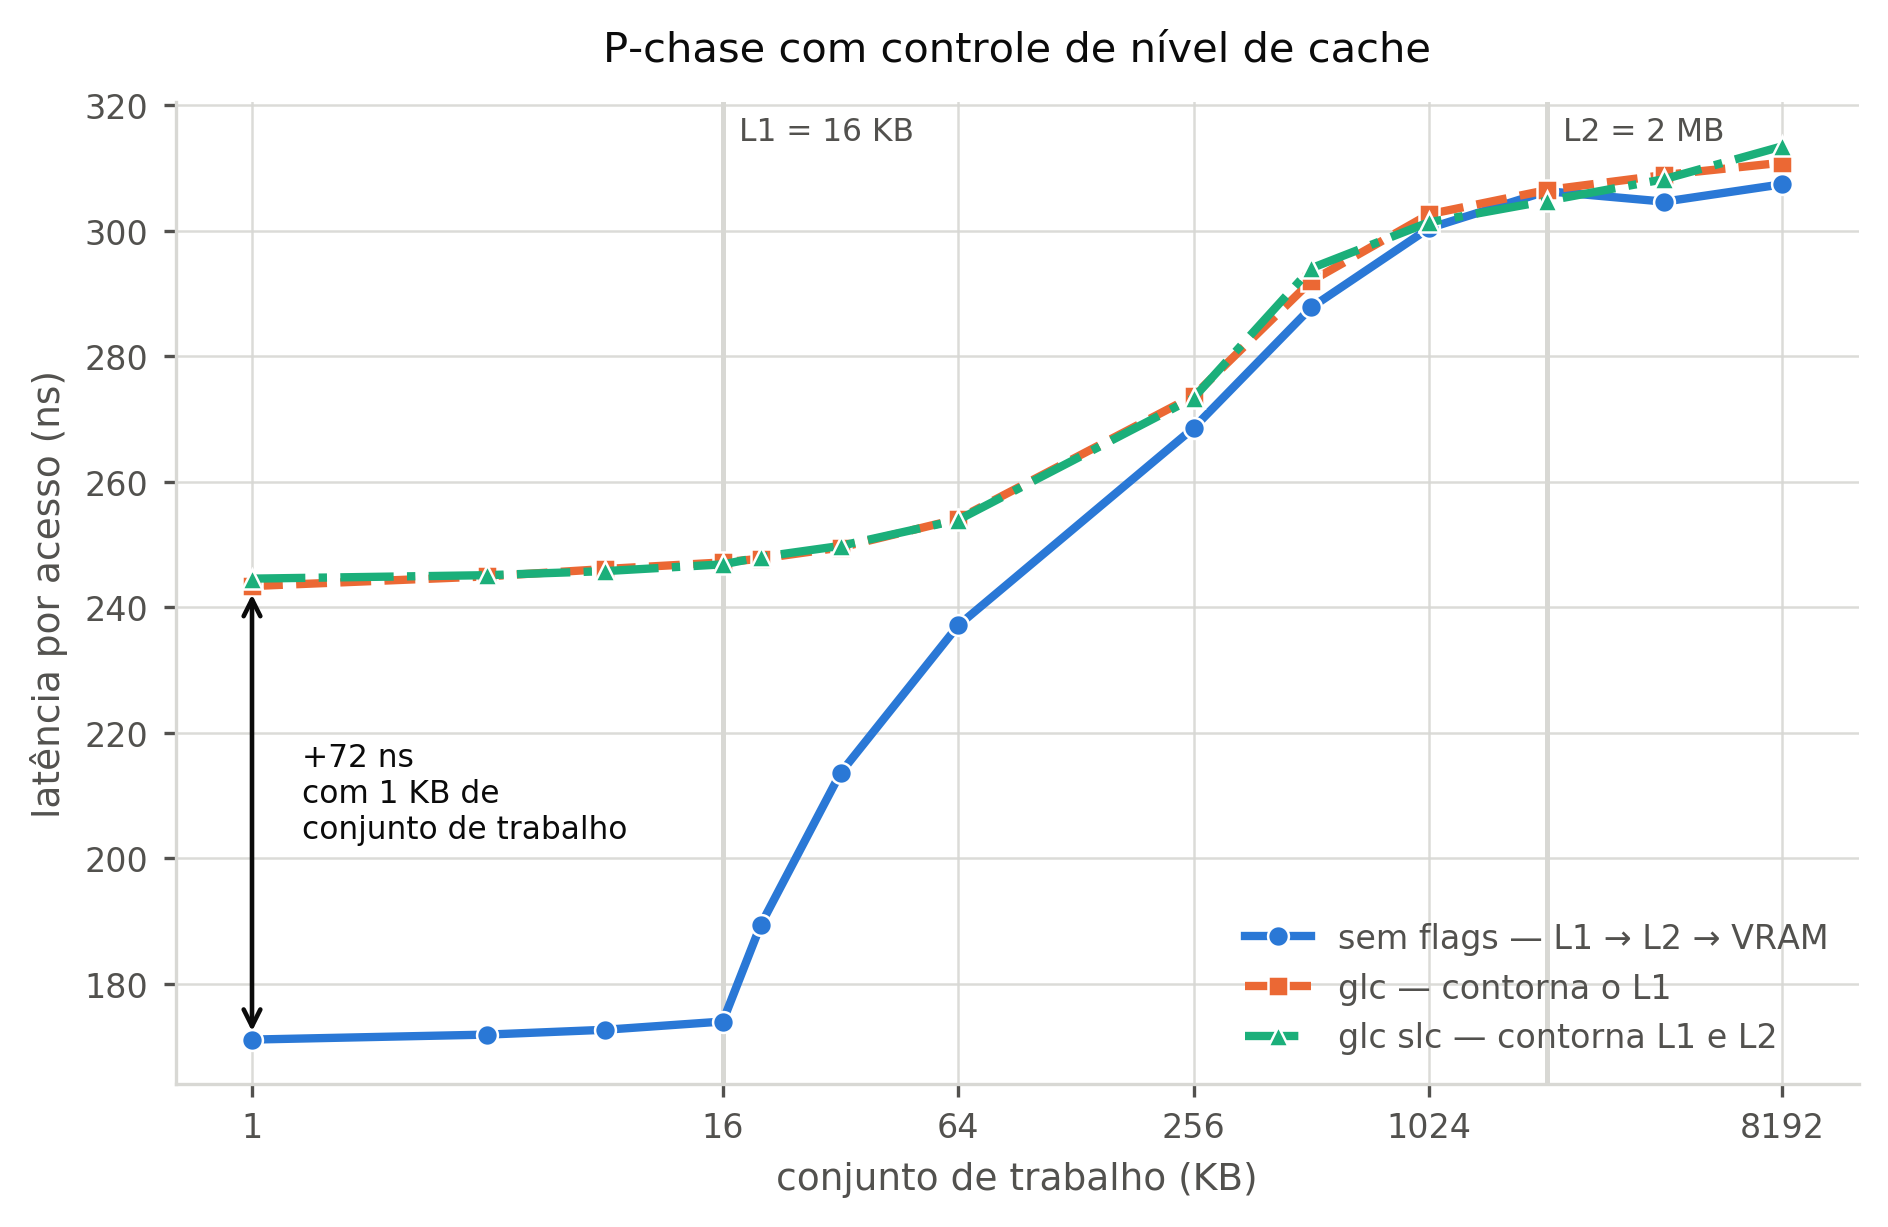
\includegraphics[width=0.66\textwidth]{fig_pchase_flags.png}
\caption{Latência de acesso em função do \textit{working set}, sob as três configurações de \textit{flags} de coerência. A curva com \texttt{glc} perde o patamar do L1; as curvas com \texttt{glc} e \texttt{glc slc} são indistinguíveis.}
\label{fig:pchase}
\end{figure}

Na curva sem \textit{flags} observa-se um patamar de 171--174~ns entre 1~KB e 16~KB, com elevação a partir de 20~KB --- o que reproduz de forma independente o tamanho do \textit{cache} L1 já obtido no Experimento~2. Na curva com \texttt{glc}, \textbf{esse patamar não existe}: com apenas 1~KB de \textit{working set}, que caberia integralmente no L1, a latência já é de 243,36~ns, um acréscimo de 72~ns (1,42$\times$). As curvas convergem a partir de aproximadamente 1~MB, como esperado, pois nesse regime o conjunto de trabalho já não cabe no L1 e contorná-lo deixa de alterar o comportamento. Confirma-se, assim, de forma direta, que a \textit{flag} \texttt{glc} contorna o \textit{cache} L1.

A comparação entre \texttt{glc} e \texttt{glc slc}, por outro lado, \textbf{refuta} a interpretação de que \texttt{slc} produza acesso direto à VRAM. As duas curvas são indistinguíveis dentro da variabilidade entre execuções: no ponto decisivo de 1~KB, quatro execuções independentes registraram diferenças entre $+0,05$\% e $+0,64$\%, sem magnitude estável. O argumento decisivo, contudo, não é a diferença entre as duas curvas, e sim a \textbf{magnitude da penalidade} de ambas. O Experimento~2, conduzido em C puro no mesmo dispositivo e sob o mesmo \textit{runtime}, mede uma penalidade de $+70$~ns na transição L1$\to$L2 (38,6~ns contra 108,7~ns) e de $+207$~ns na transição L1$\to$VRAM (38,6~ns contra 245,9~ns). A penalidade medida aqui é de $+71$~ns tanto para \texttt{glc} quanto para \texttt{glc slc}: ambas correspondem, com margem de 1~ns, à transição para o L2, e nenhuma se aproxima da transição para a VRAM. O bit é efetivamente ativado no binário (\textit{encoding} \texttt{DC530000} verificado por \textit{disassembly}), mas o acesso continua a ser servido pelo L2. Valida-se, portanto, a hipótese H2.

Esse resultado é consistente com a especificação da arquitetura, uma vez observada a distinção entre formatos de instrução. O manual do GCN3~\cite{amdgcn3} descreve o bit SLC de duas formas: para instruções MUBUF, ``\textit{when set, accesses are forced to miss in level~2 texture cache}''; para instruções FLAT --- as efetivamente emitidas pelos \textit{kernels} deste experimento --- ``\textit{used in conjunction with GLC and MTYPE to determine cache policies}'', em que MTYPE é um campo de descritor de memória sob controle do \textit{driver}, e não da instrução. A conclusão precisa não é, portanto, que \texttt{SLC=1} deixe de funcionar, e sim que \textbf{sob o formato FLAT e o MTYPE atribuído pelo \textit{runtime} OpenCL do ROCm, \texttt{SLC=1} não produz \textit{miss} no L2}. O mesmo manual corrobora diretamente o resultado obtido para \texttt{glc}: ``\textit{for GLC==1, the load intentionally misses the GPU L1 and reads from L2}''. Repetir o experimento com \texttt{buffer\_load\_dword} (MUBUF), formato para o qual a especificação promete o \textit{miss} forçado, fica registrado como encaminhamento natural deste resultado.

As latências absolutas não são comparáveis às do Experimento~2 (171~ns contra 38,6~ns para o L1), e a causa é integralmente a construção por \textit{inline assembly}: executando o \textit{kernel} de \textit{pointer chasing} em C puro sob o mesmo \textit{runtime} ROCm e o mesmo dispositivo, a latência de L1 permanece em 38,6~ns. O \textit{overhead} da construção é \textbf{aditivo e aproximadamente constante} em $125 \pm 5$~ns para \textit{working sets} de até 1~MB, o que preserva as diferenças entre níveis --- e é precisamente o que autoriza a comparação cruzada empregada no parágrafo anterior. Acima de 256~KB as medições deixam de ser reprodutíveis (variação de 10--15\% entre execuções, com inversões pontuais entre variantes); a hipótese de variação de \textit{clock} foi testada e descartada, pois a frequência permanece fixa em 1350~MHz durante toda a execução. Os valores dessa faixa não sustentam interpretação quantitativa.

\subsection{Experimento 6: Scan, Primos e Crivo}

A Tabela~\ref{tab:algoritmos} apresenta os resultados; as razões usam a mediana, robusta aos \textit{outliers} esporádicos observados em ambas as direções.

\begin{table}[ht]
\centering
\caption{Custo de contornar o L1 em três algoritmos clássicos. Todos verificados contra CPU.}
\label{tab:algoritmos}
\small
\begin{tabular}{@{}llrrr@{}}
\toprule
\textbf{Algoritmo} & \textbf{Perfil de memória} & \textbf{L1 (ms)} & \textbf{L2/L1} & \textbf{VRAM/L1} \\
\midrule
Scan & reúso $\approx$1; reúso interno no LDS & 1,423 & 1,000$\times$ & 1,003$\times$ \\
Primos & \textit{compute-bound} (controle negativo) & 1,715 & \textbf{1,000$\times$} & \textbf{1,000$\times$} \\
Crivo & dominado por escrita & 10,224 & 0,994$\times$ & 0,999$\times$ \\
\bottomrule
\end{tabular}
\end{table}

Nenhum dos três apresenta efeito mensurável, e cada um por um motivo distinto. No \textbf{scan}, o reúso global é unitário e o reúso que o algoritmo explora acontece no LDS, gerenciado explicitamente, que não passa pelo L1 --- comportamento que reproduz, num algoritmo real, o da carga sintética de \textit{streaming} da Seção~\ref{sec:niveis}.

O resultado dos \textbf{primos} tem valor metodológico: a razão é de exatamente 1,000$\times$ em ambos os níveis, com o menor desvio padrão de todo o trabalho (0,4\%). Isso demonstra que \textbf{as diferenças medidas nos demais experimentos provêm do tráfego de memória}, e não de custo intrínseco das \textit{flags} ou da construção por \textit{inline assembly} --- se tal custo existisse, apareceria aqui.

O \textbf{crivo} contrariou a previsão inicial, e o ISA explica por quê: o \textit{kernel} tem um único \texttt{flat\_load\_dword} (a tabela de primos) e um \texttt{flat\_store\_byte} por marcação. Como todos os \textit{lanes} de uma \textit{wavefront} leem o mesmo endereço da tabela, o coalescedor resolve o acesso em uma requisição por \textit{wavefront} e o tráfego de leitura torna-se desprezível; o volume concentra-se nas \textbf{escritas}, que não carregam \textit{flags} de coerência --- estas aplicam-se apenas a \textit{loads}. O crivo é, portanto, o candidato natural para investigar o comportamento das \textit{flags} em escrita.

O padrão sugerido por estes três casos é o de que o L1 só imporia custo havendo \textbf{reúso de leitura volumoso sobre conjunto de trabalho que cabe em 16~KB por CU}: reúso alto porém uniforme (crivo) não contaria; alto porém disperso (matmul, 8~MB) contaria pouco (1,27$\times$); modesto porém localizado (\textit{stencil}) contaria muito (1,80$\times$). O Experimento~7 mostra que essa formulação é \textbf{incompleta} e que a atribuição do resultado do crivo à uniformidade do acesso está equivocada: reproduzindo o mesmo padrão uniforme sobre a mesma tabela, porém com densidade de \textit{loads} três ordens de grandeza maior, o efeito reaparece.


\subsection{Experimento 7: Densidade de \textit{Loads} e a Fronteira do L1}
\label{sec:densidade}

A Tabela~\ref{tab:densidade} mostra o efeito de trocar a formulação, mantidos o problema e a verificação contra CPU.

\begin{table}[ht]
\centering
\caption{Custo de contornar o L1 por formulação do teste de primalidade. Medianas de cinco execuções independentes; dispersão entre execuções de 0,7\% (disperso), 1,5\% (crivo) e 2,7\% (uniforme). Todas as variantes verificadas contra CPU (69.581 primos em $[3{,}0;4{,}05]$~M; 513.708 em $[2^{23},2^{24})$).}
\label{tab:densidade}
\small
\begin{tabular}{@{}llrrr@{}}
\toprule
\textbf{Formulação} & \textbf{Acesso} & \textbf{\textit{Loads}} & \textbf{L1 (ms)} & \textbf{L2/L1} \\
\midrule
Crivo segmentado & uniforme & 9,2~M & 10,095 & 0,98$\times$ \\
Divisão tabelada & uniforme & 638~M & 1,481 & \textbf{2,18$\times$} \\
Divisão tabelada & disperso & 638~M & 4,163 & \textbf{7,15$\times$} \\
\bottomrule
\end{tabular}
\end{table}

O resultado \textbf{corrige a interpretação do Experimento~6}. A variante \textit{uniforme} da divisão tabelada tem exatamente o mesmo padrão de acesso do crivo --- tabela de poucos KB lida por todos os \textit{lanes} no mesmo endereço --- e ainda assim mede 2,18$\times$ contra 0,98$\times$. O que mudou não foi o padrão, e sim \textbf{quantos \textit{loads} o algoritmo emite por unidade de trabalho}: o crivo faz 2,1 escritas por \textit{load} e a divisão tabelada, 0,0016. Reúso de leitura sobre conjunto que cabe no L1 é condição \textbf{necessária, não suficiente}; falta a densidade de \textit{loads}. A dispersão atua como multiplicador sobre essa densidade, elevando o custo de 2,18$\times$ para 7,15$\times$ ao levar de 1 para até 19 o número de linhas de \textit{cache} tocadas por instrução.

Os 7,15$\times$ são o maior efeito medido neste trabalho, e o mais estável: cinco execuções independentes produziram razões entre 7,10$\times$ e 7,22$\times$, dispersão de 0,7\%. A taxa correspondente é de 44,2~G requisições/s no nível L1, ou \textbf{0,91 requisição por ciclo por CU} --- praticamente o teto arquitetural de uma requisição por ciclo por CU do L1 vetorial do GCN. O \textit{kernel} está limitado pela taxa de serviço do L1, e é por isso que retirá-lo do caminho custa tanto: a mesma taxa passa a ter de ser sustentada pelo L2, compartilhado pelas 36 CUs.

Esse ponto merece destaque por contrastar com o Experimento~5: a razão de \textbf{latência} entre L1 e L2, medida por P-chase com um único \textit{work-item}, é de apenas 1,42$\times$. Sob carga, o mesmo limite custa 7,15$\times$. A diferença mede \textbf{contenção}, e não latência --- com um único \textit{work-item} o L2 atende sem disputa; com 36 CUs saturando requisições, ele se torna o gargalo. O valor do L1 decorre, portanto, sobretudo de absorver vazão agregada, e não de encurtar o caminho de acessos individuais.

A Figura~\ref{fig:densidade} apresenta a varredura do conjunto de trabalho.

\begin{figure}[ht]
\centering
\includegraphics[width=0.98\textwidth]{fig_tdiv_ws.png}
\caption{Custo de contornar o L1 em função do conjunto de trabalho reusado. O pico ocorre em 16~KB, capacidade do L1 por CU; à direita dele o tempo \textit{com} L1 dispara, enquanto o tempo \textit{sem} L1 permanece saturado.}
\label{fig:densidade}
\end{figure}

A curva da variante dessincronizada cresce até um pico de \textbf{9,33$\times$ exatamente em 16~KB} --- a capacidade do L1 por CU --- e cai para 2,82$\times$ em 32~KB. Quatro execuções independentes reproduzem a curva com dispersão inferior a 1,3\% em todos os pontos até 32~KB. Os dois trechos medem coisas distintas. Na subida, o que se move é o numerador: abaixo de 4~KB a tabela ocupa menos de 64 linhas de \textit{cache} e os \textit{lanes} não conseguem tocar 64 linhas distintas, de modo que o tempo sem L1 dobra de $\sim$30 para $\sim$60~ms entre 4 e 8~KB e satura. Na descida, move-se o denominador: o tempo \textit{com} L1, plano em $\sim$6~ms até 16~KB, salta para 12,6~ms em 24~KB e 22,1~ms em 32~KB, à medida que o L1 deixa de reter o conjunto ativo.

O Experimento~2 localizou a fronteira dos 16~KB por latência, com um único \textit{work-item}; este experimento localiza a mesma fronteira por vazão, com a GPU saturada e sobre um algoritmo real. A convergência de dois métodos independentes sobre o mesmo limite arquitetural reforça ambos.

Um achado metodológico decorre da necessidade da terceira variante. Com as \textit{wavefronts} avançando em fase, a razão \textbf{não colapsava} após os 16~KB: permanecia em 9,40$\times$ com tabela de 51~KB. A varredura estava alterando o volume total de dados reusados, mas não o \textbf{conjunto ativo} --- o conjunto de linhas vivas simultaneamente, que é o que o \textit{cache} precisa reter. Registra-se, portanto, que em GPU o conjunto de trabalho relevante para o L1 não é o volume de dados reusados, e sim quantas linhas estão vivas ao mesmo tempo; duas cargas com o mesmo reúso sobre a mesma tabela pressionam o \textit{cache} de formas distintas conforme suas \textit{wavefronts} estejam em fase ou não.

Como limitação, manter o total de \textit{loads} constante obriga o número de \textit{work-groups} a cair de 4.882 para 191 ao longo da varredura. No último ponto restam cerca de 5,3 \textit{work-groups} por CU e, com tão poucas janelas ativas simultâneas, o conjunto ativo por CU volta a caber parcialmente no L1 --- explicação mais provável para a razão subir de 2,82$\times$ (32~KB) para 4,04$\times$ (51~KB), contra a tendência. É também o único ponto da varredura com dispersão elevada entre execuções (9,6\%, contra menos de 1,3\% nos demais), o que reforça a interpretação de instabilidade por baixa ocupação.


%% =====================================================
%% SEGUNDA RODADA DE ARQUIVAMENTO — 21/08/2026
%% Retirados ao refocar o artigo nos experimentos de controle
%% explicito das flags de cache e na varredura de tamanhos.
%% =====================================================

%% BLOCO: MET-PADROES-ACESSO

\subsection{Experimento 3: \textit{Benchmarks} de Padrões de Acesso}

São implementados \textit{benchmarks} que exercitam diferentes padrões de acesso à memória global: sequencial (contíguo, \textit{cache-friendly}), com \textit{stride} (salto fixo de 67 elementos), aleatório (\textit{xorshift}), e via memória local (LDS). Cada padrão realiza uma operação de redução sobre 16~MB de dados com 262.144 \textit{threads} e 128 iterações. Complementarmente, é implementado um \textit{stencil} 2D (\textit{blur} $3\times3$) sobre imagem $4096\times4096$, comparando acesso direto à memória global com carregamento prévio para o LDS.

%% BLOCO: MET-PCHASE

\subsection{Experimento 4: P-chase (Pointer Chasing)}

Para mapeamento direto das latências por nível de \textit{cache}, é implementado um microbenchmark baseado na técnica de \textit{pointer chasing} proposta por Wong et al.~\cite{wong2010} e refinada por Mei e Chu~\cite{mei2017}. O experimento percorre uma lista encadeada com permutação aleatória, variando o tamanho do \textit{working set} de 1~KB a 8~MB. Duas fases são conduzidas: (1)~\textit{single work-item} --- mede a latência pura sem contenção; e (2)~\textit{multi work-item} --- executa uma instância por CU (36 instâncias simultâneas), forçando contenção no L2 compartilhado e revelando a transição L2$\to$VRAM.

%% BLOCO: RES-PADROES-ACESSO

\subsection{Experimento 3: Padrões de Acesso à Memória}

A Tabela~\ref{tab:access} apresenta os resultados dos \textit{benchmarks} de redução.

\begin{table}[ht]
\centering
\caption{\textit{Benchmarks} de redução (16~MB, 262.144 \textit{threads}, 128 iterações).}
\label{tab:access}
\small
\begin{tabular}{@{}llrrl@{}}
\toprule
\textbf{Padrão de acesso} & \textbf{Tipo} & \textbf{Tempo (ms)} & \textbf{BW (GB/s)} & \textbf{Razão} \\
\midrule
Sequencial (contíguo) & \textit{cache-friendly} & 0,35 & 383 & 1,0$\times$ \\
LDS (memória local) & \textit{cache-friendly} & 0,34 & 396 & 1,03$\times$ \\
\textit{Stride} (salto 67) & \textit{cache-hostile} & 17,94 & 7,5 & 0,020$\times$ \\
Aleatório (\textit{xorshift}) & \textit{cache-hostile} & 18,03 & 7,4 & 0,019$\times$ \\
\bottomrule
\end{tabular}
\end{table}

A diferença de $\sim$51$\times$ na \textit{bandwidth} efetiva entre o acesso sequencial (383~GB/s) e o aleatório (7,4~GB/s) evidencia o impacto da hierarquia de \textit{cache}: ambos os padrões utilizam as mesmas instruções ISA (GLC=0, SLC=0), mas a taxa de \textit{cache miss} difere drasticamente em função da localidade espacial.

Convém explicitar como esse número deve ser lido. Trata-se de \textit{bandwidth} efetiva, calculada sobre o volume de dados logicamente lido pelo algoritmo, e não do tráfego que efetivamente chega à VRAM. O Experimento~7 mede diretamente o teto da memória global desta placa em 222~GB/s; os 383~GB/s do padrão sequencial estão acima desse teto justamente porque as 128 iterações reencontram nos \textit{caches} parte dos dados já lidos. O contraste de 51$\times$ permanece válido como medida do impacto da localidade, mas nenhum dos dois valores deve ser interpretado como vazão de VRAM.

No \textit{stencil} 2D (\textit{blur} $3\times3$, imagem $4096\times4096$), o acesso via memória global (0,71~ms) foi mais rápido que a versão com LDS (0,85~ms), indicando que o \textit{cache} L1 é suficientemente eficiente para padrões com alta localidade espacial, não justificando o \textit{overhead} de carregamento e sincronização do LDS.

%% BLOCO: RES-PCHASE

\subsection{Experimento 4: P-chase}

A Tabela~\ref{tab:pchase} resume os resultados do P-chase em modo \textit{single work-item} (latência pura, sem contenção entre CUs).

\begin{table}[ht]
\centering
\caption{Latência por \textit{working set} (P-chase, \textit{single work-item}).}
\label{tab:pchase}
\small
\begin{tabular}{@{}rrl@{}}
\toprule
\textbf{Working Set} & \textbf{Latência (ns)} & \textbf{Nível inferido} \\
\midrule
1--16 KB & $\sim$39 & L1 \\
20 KB & $\sim$59 (+52\%) & Transição L1$\to$L2 \\
32--512 KB & 86--140 & L2 \\
1--8 MB & $\sim$137 & VRAM \\
\bottomrule
\end{tabular}
\end{table}

O salto de latência em 20~KB confirma experimentalmente que o \textit{cache} L1 da Ellesmere possui 16~KB por CU, consistente com a especificação da AMD. No modo \textit{multi work-item} (36 instâncias, uma por CU), a transição L2$\to$VRAM torna-se visível: a latência salta de 203~ns (\textit{working set} de 64~KB/CU, \textit{footprint} total de 2,3~MB $\approx$ L2) para 301~ns (256~KB/CU, \textit{footprint} de 9~MB $\gg$ L2), um aumento de $\sim$48\%. A VRAM sob contenção real (36 CUs simultâneos) apresenta latência 2,3$\times$ maior que no teste com 1 \textit{work-item}, evidenciando o efeito da contenção no barramento de memória.


%% =====================================================
%% TERCEIRA RODADA DE ARQUIVAMENTO — 11/09/2026
%% Comparativo Windows x Linux retirado do texto e reservado
%% para a apresentacao a banca. Restou uma linha na metodologia.
%% =====================================================

%% BLOCO: MET-AMBIENTE-DOIS-SO

Os experimentos são conduzidos em uma GPU AMD Ellesmere (RX 580 8~GB, arquitetura GCN 4\textordfeminine{} geração, GFX8) com 36 \textit{Compute Units} a 1350~MHz, \textit{cache} L1 de 16~KB por CU (\textit{write-through}), \textit{cache} L2 de 2~MB compartilhado, LDS de 64~KB por CU e 8~GB de VRAM GDDR5. O mesmo dispositivo físico é acessado
a partir de dois ambientes de software, em \textit{dual boot}: com isso o
\textit{hardware} permanece constante e a pilha de compilação é a única variável
entre eles. A Tabela~\ref{tab:ambiente} descreve os dois ambientes; a metodologia
compreende cinco experimentos, distribuídos entre eles conforme a última linha
da tabela.

%% BLOCO: TAB-AMBIENTE

\begin{table}[ht]
\centering
\caption{Ambientes de execução. O dispositivo é o mesmo nos dois; varia apenas a
pilha de software.}
\label{tab:ambiente}
\small
\begin{tabular}{@{}lll@{}}
\toprule
 & \textbf{Ambiente Windows} & \textbf{Ambiente Linux} \\
\midrule
Sistema operacional & Windows~11 & Ubuntu, \textit{kernel} 5.15 \\
\textit{Runtime} OpenCL & AMD Adrenalin (OpenCL~1.2) & ROCm~5.2$^\ast$ \\
Compilador de \textit{kernel} & AMDOCL (proprietário) & Clang/LLVM (\texttt{comgr}) \\
Compilador \textit{host} & MinGW GCC & GCC \\
Desmontagem de ISA & decodificador próprio, \texttt{clrxdisasm}, RGA & \texttt{llvm-objdump} \\
\textit{Runtimes} adicionais & --- & Mesa Clover, PoCL \\
Experimentos & 1 & 2 a 5 \\
\bottomrule
\end{tabular}

\vspace{2pt}
{\footnotesize $^\ast$ A arquitetura Polaris é depreciada no ROCm~5.2 e o
dispositivo só é enumerado com \texttt{ROC\_ENABLE\_PRE\_VEGA=1}.}
\end{table}

%% BLOCO: MET-EXP1-WINDOWS

\subsection{Experimento 1: Antecedentes --- \texttt{volatile} e Análise ISA em Windows}

Quatro \textit{kernels} de multiplicação de matrizes $1024 \times 1024$ avaliam a
hipótese inicial do trabalho: que o qualificador \texttt{volatile} forçaria o
\textit{bypass} do L1 pela \textit{flag} GLC. As variantes são o acesso padrão, duas
com \texttt{volatile} em graus distintos e uma \textit{tiled} com memória local.

Para verificar se o qualificador de fato altera as instruções emitidas, o binário
compilado pelo \textit{driver} é extraído via
\texttt{clGetProgramInfo(CL\_PROGRAM\_BINARIES)} e desmontado por duas ferramentas
independentes: um decodificador próprio, em C++, que percorre a estrutura ELF
aninhada do binário e extrai os campos GLC e SLC, e o CLRadeonExtender
(\texttt{clrxdisasm}). O Radeon GPU Analyzer (RGA) compila os mesmos
\textit{kernels} \textit{offline}, o que isola a variável ``ambiente de execução''.
Investigam-se ainda mecanismos alternativos de controle direto: \textit{inline
assembly} GCN, edição dos bits GLC/SLC no binário (\textit{binary patching}) e o
HIP SDK da AMD.

%% BLOCO: RES-EXP1-WINDOWS

\subsection{Experimento 1: Antecedentes --- \texttt{volatile} e Análise ISA em Windows}

Sob o \textit{driver} Windows, a variante normal e as duas com \texttt{volatile}
produziram tempos indistinguíveis ($\sim$6,2~ms, $\sim$346~GFLOPS), enquanto a
\textit{tiled} com memória local foi cerca de três vezes mais rápida (2,07~ms,
1.038~GFLOPS). A análise de ISA explica o empate: as ferramentas convergem em que
todos os \textit{kernels}, com e sem o qualificador, geram \texttt{DC500000} ---
\texttt{flat\_load\_dword} com GLC=0. O \texttt{volatile} não é ignorado: atua como
barreira de otimização, impedindo o reuso de valores em registradores (10 contra
11 VGPRs) e a reordenação de \textit{loads}; sob esse compilador, porém, a barreira
não se traduz em \textit{flags} de \textit{cache}.

A compilação \textit{offline} para o mesmo \textit{target} reproduz o resultado, o
que afasta o \textit{driver} e o sistema operacional como responsáveis pela ausência
de \textit{flags}. Para \textit{targets} posteriores (gfx900, gfx950) o mesmo fonte
passa a gerar \texttt{glc} e \texttt{sc0 sc1}, o que sugere decisão de
\textit{codegen}; como as versões do RGA diferem entre alvos, porém, essa comparação
isolada não separa arquitetura de evolução do \textit{backend} --- questão que o
Experimento~2 resolve de forma direta.

Nenhum mecanismo alternativo se mostrou viável neste ambiente: o \textit{inline
assembly} produz GLC=1 (\texttt{DC510000}) na compilação \textit{offline},
confirmando que a instrução existe na ISA do GFX8, mas o AMDOCL não reconhece a
sintaxe \texttt{\_\_asm\_\_}; o \textit{binary patching} é carregado pelo
\textit{driver} e falha na execução, por inconsistência dos metadados HSA; e o HIP
SDK para Windows exige no mínimo RDNA2. Em GFX8/OpenCL/Windows, portanto,
\textbf{não existe mecanismo suportado para controle de \textit{cache} em tempo de
execução} --- e o \textit{kernel} nomeado \texttt{matmul\_direto\_VRAM} não realiza
acesso direto à VRAM: gera código idêntico ao \texttt{matmul\_via\_L2}, refletindo a
expectativa corrente sobre as \textit{flags} e não o que a ISA oferece.
